\documentclass[border=10pt]{standalone}

\usepackage[utf8]{inputenc}
\usepackage[english]{babel}
\usepackage{tikz}
\usepackage{graphicx}
\usepackage{subfigure}

\usepackage{pgfplots}
\pgfplotsset{compat=1.15}

\begin{document}

	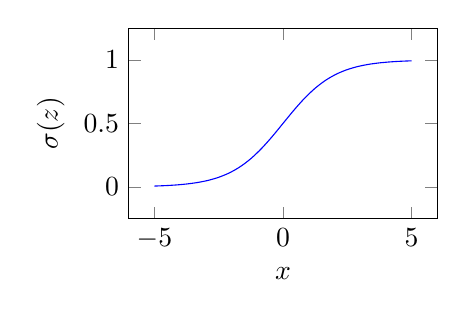
\begin{tikzpicture}
		\begin{axis}[width=5.5cm,height=4cm,ylabel=$\sigma(z)$,xlabel=$x$,ymin=-0.25,ymax=1.25,xmin=-6,xmax=6]
			\addplot[blue,smooth] {1/(1+exp(-x))};
		\end{axis}
	\end{tikzpicture}
	
	
	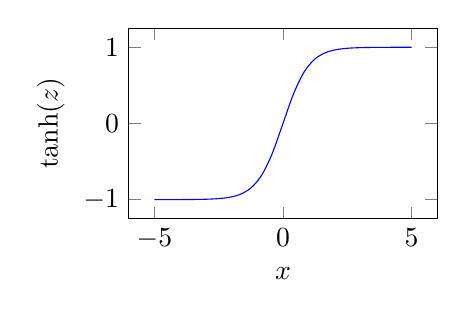
\begin{tikzpicture}
		\begin{axis}[width=5.5cm,height=4cm,ylabel=$\tanh(z)$,xlabel=$x$,ymin=-1.25,ymax=1.25,xmin=-6,xmax=6]
			\addplot[blue,smooth] {tanh(x)};
		\end{axis}
	\end{tikzpicture}
	
	
	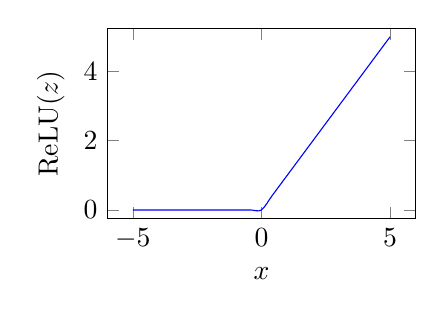
\begin{tikzpicture}
		\begin{axis}[width=5.5cm,height=4cm,ylabel=$\textnormal{ReLU}(z)$,xlabel=$x$,ymin=-0.25,ymax=5.25,xmin=-6,xmax=6]
			\addplot[blue,smooth] {max(0,x)};
		\end{axis}
	\end{tikzpicture}
	
\end{document}